% \begin{document}

\chapter{Dining Philosophers}

Dining philosophers is a famous problem used to illustrate concurrent algorithm
design \cite{dining}. The problem states there are N philosophers sitting in a
circle, with a fork placed between each philosopher. This is illustrated
below:\\

\begin{center}
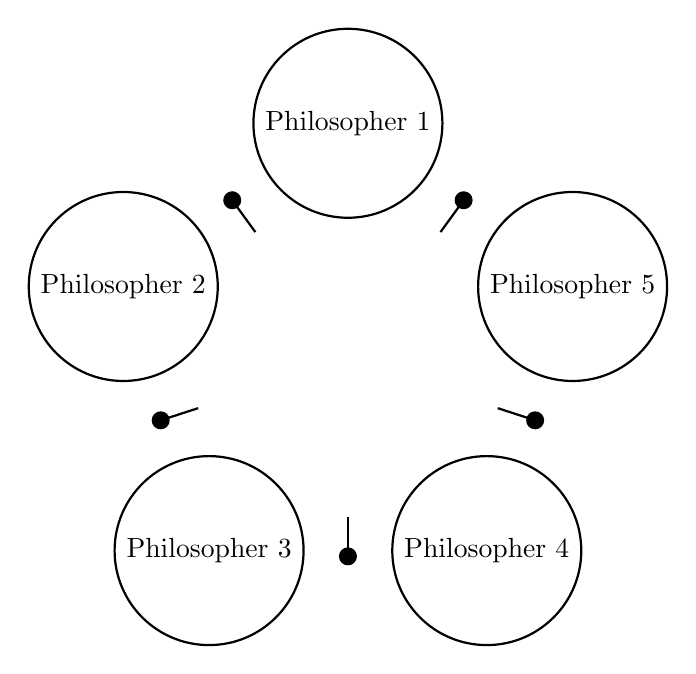
\begin{tikzpicture}

    % Draw the philosophers
    \foreach \angle/\name in {90/Philosopher 1, 162/Philosopher 2, 234/Philosopher 3, 306/Philosopher 4, 18/Philosopher 5} {
        \draw[thick] (\angle:3cm) circle (1.2cm); % Larger circle for philosophers
        \node at (\angle:3cm) {\name}; % Philosopher label
    }

    % Draw the forks between the philosophers
    \foreach \angle in {126, 198, 270, 342, 54} {
        \draw[thick] (\angle:2cm) -- (\angle:2.5cm); % Fork handle
        \draw[thick, fill=black] (\angle:2.5cm) circle (0.1cm); % Fork tip
    }

\end{tikzpicture}
\end{center}

Each philosopher is either thinking or eating, but the philosopher needs to take
\textit{both} forks to eat. The problem is to design a solution that ensures one
or more philosophers can eat when they want to. \\

A possible failing scenario is when \textit{all} philosophers take the fork to
their left. Now every philosopher is stuck waiting for the fork to their right, 
and every philosopher starve.

\section{Design}

Every philosopher behaves similarly:
\begin{itemize}
    \item Take one fork 
    \item Take another fork 
    \item Eat
    \item Put away one fork
    \item Put away another fork
\end{itemize}

\section{Spec}

The core part of \textit{Spec} looks like this: 
\\
\begin{tla}
Next ==
    \/ \E k \in 0.. P-1:
        TakeFirst(k)
    \/ \E k \in 0.. P-1:
        TakeSecond(k)
    \/ \E k \in 0.. P-1:
        Eat(k)
    \/ \E k \in 0.. P-1:
        PutFirst(k)
    \/ \E k \in 0.. P-1:
        PutSecond(k)
\end{tla}
\begin{tlatex}
\@x{ Next \.{\defeq}}%
\@x{\@s{16.4} \.{\lor} \E\, k \.{\in} 0 \.{\dotdot} P \.{-} 1 \.{:}}%
\@x{\@s{20.5} TakeFirst ( k )}%
\@x{\@s{16.4} \.{\lor} \E\, k \.{\in} 0 \.{\dotdot} P \.{-} 1 \.{:}}%
\@x{\@s{20.5} TakeSecond ( k )}%
\@x{\@s{16.4} \.{\lor} \E\, k \.{\in} 0 \.{\dotdot} P \.{-} 1 \.{:}}%
\@x{\@s{20.5} Eat ( k )}%
\@x{\@s{16.4} \.{\lor} \E\, k \.{\in} 0 \.{\dotdot} P \.{-} 1 \.{:}}%
\@x{\@s{20.5} PutFirst ( k )}%
\@x{\@s{16.4} \.{\lor} \E\, k \.{\in} 0 \.{\dotdot} P \.{-} 1 \.{:}}%
\@x{\@s{20.5} PutSecond ( k )}%
\end{tlatex}
\\

This reflects the behavior described earlier. Note that there's a sequential
dependency to these actions. The philosopher can only take the second fork after
taking the first fork, eat after having both forks and put away the forks after
eating.\\

\begin{tla}

First(k) == k
Second(k) == (k+1)% P

TakeFirst(k) == 
    /\ eaten[k] = 0
    /\ forks[First(k)] = UNUSED
    /\ UNCHANGED eaten

TakeSecond(k) ==
    /\ eaten[k] = 0
    /\ forks[First(k)] = k
    /\ forks[Second(k)] = UNUSED
    /\ forks' = [forks EXCEPT ![Second(k)] = k]
    /\ UNCHANGED eaten
\end{tla}
\begin{tlatex}
\@x{ First ( k ) \.{\defeq} k}%
\@x{ Second ( k ) \.{\defeq} ( k \.{+} 1 ) \.{\%} P}%
\@pvspace{8.0pt}%
\@x{ TakeFirst ( k ) \.{\defeq}}%
\@x{\@s{16.4} \.{\land} eaten [ k ] \.{=} 0}%
\@x{\@s{16.4} \.{\land} forks [ First ( k ) ] \.{=} UNUSED}%
\@x{\@s{16.4} \.{\land} {\UNCHANGED} eaten}%
\@pvspace{8.0pt}%
\@x{ TakeSecond ( k ) \.{\defeq}}%
\@x{\@s{16.4} \.{\land} eaten [ k ] \.{=} 0}%
\@x{\@s{16.4} \.{\land} forks [ First ( k ) ] \.{=} k}%
\@x{\@s{16.4} \.{\land} forks [ Second ( k ) ] \.{=} UNUSED}%
 \@x{\@s{16.4} \.{\land} forks \.{'} \.{=} [ forks {\EXCEPT} {\bang} [ Second
 ( k ) ] \.{=} k ]}%
\@x{\@s{16.4} \.{\land} {\UNCHANGED} eaten}%
\end{tlatex}
\\

The philosopher greedily takes the first fork when possible. After the
philosopher has the first fork, she greedily takes the second fork when
possible.
\\

\begin{tla}
Eat(k) == 
    LET 
        left == k 
        right == (k+1) % P
    IN 
        /\ forks[left] = k
        /\ forks[right] = k
        /\ eaten' = [eaten EXCEPT ![k] = 1]
        /\ UNCHANGED forks 
\end{tla}
\begin{tlatex}
\@x{ Eat ( k ) \.{\defeq}}%
\@x{ \.{\LET}}%
\@x{\@s{16.4} left \.{\defeq} k}%
\@x{\@s{16.4} right \.{\defeq} ( k \.{+} 1 ) \.{\%} P}%
\@x{ \.{\IN}}%
\@x{\@s{16.4} \.{\land} forks [ left ] \.{=} k}%
\@x{\@s{16.4} \.{\land} forks [ right ] \.{=} k}%
 \@x{\@s{16.4} \.{\land} eaten \.{'} \.{=} [ eaten {\EXCEPT} {\bang} [ k ]
 \.{=} 1 ]}%
\@x{\@s{16.4} \.{\land} {\UNCHANGED} forks}%
\end{tlatex}
\\

Once the philosopher has both forks, she can eat. 
\\
\begin{tla}
PutFirst(k) == 
    /\ eaten[k] = 1
    /\ forks[First(k)] = k 
    /\ forks' = [forks EXCEPT ![First(k)] = UNUSED]
    /\ UNCHANGED eaten

PutSecond(k) == 
    /\ eaten[k] = 1
    /\ forks[First(k)] # k 
    /\ forks[Second(k)] = k 
    /\ forks' = [forks EXCEPT ![Second(k)] = UNUSED]
    /\ eaten' = [eaten EXCEPT ![k] = 0]
\end{tla}
\begin{tlatex}
\@x{ PutFirst ( k ) \.{\defeq}}%
\@x{\@s{16.4} \.{\land} eaten [ k ] \.{=} 1}%
\@x{\@s{16.4} \.{\land} forks [ First ( k ) ] \.{=} k}%
 \@x{\@s{16.4} \.{\land} forks \.{'} \.{=} [ forks {\EXCEPT} {\bang} [ First (
 k ) ] \.{=} UNUSED ]}%
\@x{\@s{16.4} \.{\land} {\UNCHANGED} eaten}%
\@pvspace{8.0pt}%
\@x{ PutSecond ( k ) \.{\defeq}}%
\@x{\@s{16.4} \.{\land} eaten [ k ] \.{=} 1}%
\@x{\@s{16.4} \.{\land} forks [ First ( k ) ] \.{\neq} k}%
\@x{\@s{16.4} \.{\land} forks [ Second ( k ) ] \.{=} k}%
 \@x{\@s{16.4} \.{\land} forks \.{'} \.{=} [ forks {\EXCEPT} {\bang} [ Second
 ( k ) ] \.{=} UNUSED ]}%
 \@x{\@s{16.4} \.{\land} eaten \.{'} \.{=} [ eaten {\EXCEPT} {\bang} [ k ]
 \.{=} 0 ]}%
\end{tlatex}
\\

After eating, the philosopher puts away the forks.

\section{Safety}

Omitted for this chapter.

\section{Liveness}

One liveness property is to ensure that at least one philosopher can eat when she
wants to under all circumstances:\\

\begin{tla}
Liveness ==
    \E k \in 0..P-1:
        /\ eaten[k] = 0 ~> eaten[k] = 1
        /\ eaten[k] = 1 ~> eaten[k] = 0
\end{tla}
\begin{tlatex}
\@x{ Liveness \.{\defeq}}%
\@x{\@s{16.4} \E\, k \.{\in} 0 \.{\dotdot} P \.{-} 1 \.{:}}%
\@x{\@s{20.5} \.{\land} eaten [ k ] \.{=} 0 \.{\leadsto} eaten [ k ] \.{=} 1}%
\@x{\@s{20.5} \.{\land} eaten [ k ] \.{=} 1 \.{\leadsto} eaten [ k ] \.{=} 0}%
\end{tlatex}
\\

However, \textit{Spec} defined as is doesn't implement any deadlock mitigation.
Running it against the model the checker results in the following violations: 

\begin{verbatim}
State 2: <TakeFirst line 19, col 5 to line 23, 
    col 22 of module dining>
/\ eaten = (0 :> 0 @@ 1 :> 0 @@ 2 :> 0)
/\ forks = (0 :> 0 @@ 1 :> 100 @@ 2 :> 100)

State 3: <TakeFirst line 19, col 5 to line 23, 
    col 22 of module dining>
/\ eaten = (0 :> 0 @@ 1 :> 0 @@ 2 :> 0)
/\ forks = (0 :> 0 @@ 1 :> 1 @@ 2 :> 100)

State 4: <TakeFirst line 19, col 5 to line 23, 
    col 22 of module dining>
/\ eaten = (0 :> 0 @@ 1 :> 0 @@ 2 :> 0)
/\ forks = (0 :> 0 @@ 1 :> 1 @@ 2 :> 2)
\end{verbatim}

When all philosopher takes their left fork, no one can eat. \\

A simple fix to the problem is for every philosopher to take the fork with the
smaller index first:\\

\begin{tla}
First(k) == IF k # P-1 THEN k ELSE 0
Second(k) == IF k # P-1 THEN k+1 ELSE k
\end{tla}
\begin{tlatex}
 \@x{ First ( k ) \.{\defeq} {\IF} k \.{\neq} P \.{-} 1 \.{\THEN} k \.{\ELSE}
 0}%
 \@x{ Second ( k ) \.{\defeq} {\IF} k \.{\neq} P \.{-} 1 \.{\THEN} k \.{+} 1
 \.{\ELSE} k}%
\end{tlatex}
\\

When the philosopher with the highest index wants to eat, she will need to take
fork 0 first. In the case where all other philosophers have already taken their
first fork, the philosopher with the highest index will fail to take her first
fork (because it has already been taken by the first philosopher). This allows
the philosopher with the second-highest index to make progress, thus preventing a
deadlock.\\

The model checker will pass the updated \textit{Spec}.

% \end{document}
